\documentclass{article}
\usepackage[utf8]{inputenc}
\usepackage{graphicx} 

\title{miniproject write up}
\author{kate.griffin21 }
\date{December 2021}

\begin{document}
\maketitle
\newpage
\tableofcontents
\newpage
\section{Introduction}
\begin{flushleft}

Food spoilage may be defined as any change in a food product which deems it unsuitable for consumption by a consumer \cite{bae2014growth}. The most common cause of food spoilage is that caused by microbes, which can alter a food item’s flavour, smell, texture and taste \cite{bae2014growth}. The surfaces of food products are often nutrient rich and, in combination with suitable environmental conditions, this can facilitate the growth of biofilms \cite{bae2014growth}. In the food industry, predicting microbial growth may be useful in evaluating risk and shelf life of perishable goods \cite{huang2013optimization}\cite{bae2014growth}\cite{zwietering1990modeling}. Microbial growth rates may be measured by plotting population density against time on a graph and fitting a straight line through the exponential growth phase. The slope of this line represents the maximum growth rate (r max). In recent years, predictive microbiologists use mathematical models which can describe the growth of microorganisms along the sigmoidal bacterial growth curve. Such models include the Gompertz (cite), Logistic (cite), Baranyi and Buchanan models\cite{huang2013optimization}.
\linebreak

The growth of a bacteria in batch culture may be divided into five main phases based on the slope of its growth curve \cite{rolfe2012lag}\cite{huang2013optimization}\cite{finkel2006long}\cite{zwietering1990modeling}. The first phase is the lag phase, where bacteria adapt themselves in preparation for their growth. During this phase, a number of genes are activated, including those involved in the uptake of nutrients, DNA repair, RNA processing, cell division and other biomolecular processes. The next phase is the exponential growth phase, where cell division occurs at a constant rate following a geometric progression. Once carrying capacity of the environment (i.e., growing media) has been reached, the stationary phase commences. During this phase, bacteria stop replicating. The next phase is the death phase, which occurs when the bacterial cells lose viability. The last stage is the long-term stationary phase,  where bacteria can remain for long periods of time without nutrients \cite{finkel2006long}.
\linebreak


Ecological and evolutionary models may be considered as a spectrum between phenomenological to mechanistic methods \cite{white2019should}. Models may be described as mechanistic if they include a number of parameters with biological definitions, which may be measured independently of the observed data \cite{transtrum2016bridging}\cite{white2019should}. In comparison, phenomenological models (e.g., cubic and quadratic polynomial models) measure a hypothesised relationship between two or more variables in a dataset, which can be fitted to the data \cite{white2019should}. When applied to measure population growth, the logistic model takes the carrying capacity of the environment into account. It demonstrates that the per capita growth rate decreases as population density increases \cite{stefan2012mathematical}. This is because populations grow exponentially while their population size is low and resources are not limiting, and then slows down as the population becomes so large that resources become limited (i.e., the Malthusian principle). The logistic model may be considered a mechanistic model when modelling population size, as it can be modified to include parameters which have biological meaning.
\linebreak


Although mechanistic models are more robust than phenomenological models, they are not necessarily more valuable in making predictions \cite{white2019should}. Mechanistic models are particularly suitable for analysing populations when predictions outside of the known set of parameters is required and there is also enough existing data to make a priori estimates of its parameters \cite{white2019should}. When a biological system or processes can be explained by relatively few variables, a simpler model with fewer parameters may be more useful \cite{transtrum2016bridging}.The aim of my analysis is to address the question as to whether phenomenological models or logistic models are better for modelling population growth in microbial batch cultures. In my analysis I will be comparing a quadratic polynomial model to a mechanistic logistic model in predicting the change in microbe abundance over time.

\newpage
\section{Methods}
\subsection{Preparing the data}
The dataset used in this analysis contains measurements of biomass/number of cells of forty-five species of microbes grown on eighteen different media over time. The data was collected from ten different studies across the world. Field names are defined in the metadata file. The two main variables I will be comparing are “PopBio” (abundance) and “Time”. Single population growth curves were identified as unique combinations of temperature, growing media, species and citation. These unique IDs were saved in a new column and used to subset the data. The data was wrangled in Python. Firstly, the data was checked for NA values as well as negative values for PopBio and Time. Rows which contained negative values were deleted. There were no NA values found in the dataset. The wrangled data with the unique ID column was then saved as a .csv file.
\linebreak

\subsection{Fitting the models}
The models were defined and ran in R. The models were fit in order to find their estimated parameters. AIC and BIC were then calculated to find the fit of the model parameters to the observed data. The first model fitted was the polynomial quadratic model, the equation for which is:

\[B = B\textsubscript{0}+B\textsubscript{1}x+B\textsubscript{2}x\textsuperscript{2}\]

where x represents an independent variable, which in this analysis is time. B\textsubscript{0}, B\textsubscript{1}, B\textsubscript{2} represents the parameters, i.e., the coefficients of the equation (respectively: the quadratic coefficient, the linear coefficient and the constant or term). Once the model was defined, it was ran on each subset of data. The AIC and BIC were calculated and saved.
\linebreak

The next model to be fit was the logistic model, the classic  equation for which is:

\[Nt = \frac{N\textsubscript{0} K e\textsuperscript{rt}}{K + N\textsubscript{0} (e\textsuperscript{rt} - 1)}\]

The three parameters defined in the model are: r (maximum growth rate, also known as R max), K (carrying capacity) and N\textsubscript{0} (initial population). Nt represents the population size at time t, and No is the initial population size. As with the quadratic model, the model was fit to find its parameters and ran on each subset. AIC and BIC were calculated to evaluate the fit.

\subsection{Plotting and analysis}

The difference in AIC between the quadratic and the logistic model was calculated for each subset. If the absolute difference was greater than 2, then the model with the smaller AIC value was selected as the better model. I created a tally of the models selected for each subset to compare which model was selected more often based on AIC. BIC was also then compared using the same method as AIC. Plots were created to visualise the fit of the models against the observed data as well as the tally of the most suitable model.

\newpage
\section{Results}
The results of the AIC and BIC analysis suggested that the quadratic model was better at predicting the growth of microbes more often than the logistic model. 


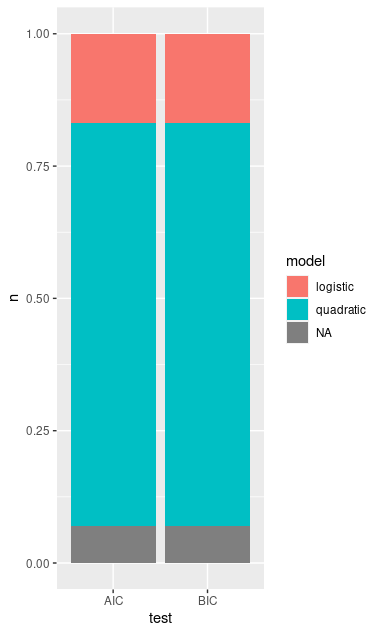
\includegraphics[width=10cm,height=10cm,keepaspectratio]{best_model.png}



\bibliographystyle{plain}

\bibliography{FirstBiblio}

\end{flushleft}
\end{document}
